%=======================================================================
%  feynman_explainer.tex
%  A from-scratch, Feynman-style explanation of the paper:
%  "Fusing Two-Stage LLM Semantic Refinement with Genetic Programming
%   for Robust Alpha Discovery and Degradation Mitigation" (IEEE Access)
%
%  BUILD (from this folder):
%     pdflatex -interaction=nonstopmode feynman_explainer.tex
%     pdflatex -interaction=nonstopmode feynman_explainer.tex
%=======================================================================
\documentclass[11pt,a4paper]{article}

% ------------------------------- packages ----------------------------
\usepackage[T1]{fontenc}
\usepackage[utf8]{inputenc}
\usepackage{lmodern}
\usepackage{microtype}
\usepackage[margin=2.4cm]{geometry}
\usepackage{amsmath,amssymb,amsthm}
\usepackage{booktabs}
\usepackage{multirow}
\usepackage{tabularx}
\usepackage{array}
\usepackage{graphicx}
\usepackage{xcolor}
\usepackage{enumitem}
\usepackage{caption}
\usepackage{tcolorbox}
\usepackage{hyperref}
\usepackage{float}

\tcbuselibrary{skins,breakable}

% ------------------------------- colours -----------------------------
\definecolor{ink}{HTML}{1A1A2E}
\definecolor{feyn}{HTML}{0B6E4F}
\definecolor{feynlight}{HTML}{E8F5EF}
\definecolor{warn}{HTML}{B3541E}
\definecolor{warnlight}{HTML}{FDF1E7}
\definecolor{mathbg}{HTML}{F1F4F9}
\definecolor{rule}{HTML}{C9D6E3}
\definecolor{navy}{HTML}{0E2A47}
\definecolor{accent}{HTML}{0091B3}

\hypersetup{
  colorlinks=true, linkcolor=navy, citecolor=feyn,
  urlcolor=accent,
  pdftitle={Feynman-Style Explanation of the Two-Stage LLM Semantic Refinement Paper}
}

% ------------------------- custom environments ----------------------
\newtcolorbox{plaineng}[1][Plain English]{%
  enhanced, breakable, colback=feynlight, colframe=feyn,
  title={\bfseries #1}, fonttitle=\small,
  attach boxed title to top left={xshift=4pt,yshift=-3pt},
  boxed title style={colback=feyn, colframe=feyn, sharp corners},
  sharp corners, arc=2pt, left=6pt, right=6pt, top=4pt, bottom=4pt,
  boxrule=0.6pt, before skip=8pt, after skip=8pt
}

\newtcolorbox{scrutiny}[1][Feynman's Rule: Do Not Fool Yourself]{%
  enhanced, breakable, colback=warnlight, colframe=warn,
  title={\bfseries #1}, fonttitle=\small,
  attach boxed title to top left={xshift=4pt,yshift=-3pt},
  boxed title style={colback=warn, colframe=warn, sharp corners},
  sharp corners, arc=2pt, left=6pt, right=6pt, top=4pt, bottom=4pt,
  boxrule=0.6pt, before skip=8pt, after skip=8pt
}

\newtcolorbox{themath}[1][The Math (When You Are Ready)]{%
  enhanced, breakable, colback=mathbg, colframe=navy,
  title={\bfseries #1}, fonttitle=\small,
  attach boxed title to top left={xshift=4pt,yshift=-3pt},
  boxed title style={colback=navy, colframe=navy, sharp corners},
  sharp corners, arc=2pt, left=6pt, right=6pt, top=4pt, bottom=4pt,
  boxrule=0.6pt, before skip=8pt, after skip=8pt
}

\newcommand{\takeaway}[1]{\noindent\fcolorbox{feyn}{feynlight}{\parbox{\dimexpr\linewidth-2\fboxsep-2\fboxrule}{\textbf{Takeaway.} #1}}\par\medskip}

\newcommand{\code}[1]{\texttt{#1}}

\captionsetup{font=small, labelfont=bf}

\setlist[itemize]{leftmargin=1.2em, itemsep=2pt, topsep=2pt}
\setlist[enumerate]{leftmargin=1.6em, itemsep=2pt, topsep=2pt}

%=======================================================================
\begin{document}

\begin{center}
  {\LARGE\bfseries\color{navy} The Paper, Explained from Scratch}\\[6pt]
  {\large\color{ink} A Feynman-Style Walkthrough of ``Fusing Two-Stage LLM Semantic\\
  Refinement with Genetic Programming for Robust Alpha Discovery\\
  and Degradation Mitigation''}\\[8pt]
  {\small A first-principles companion to the manuscript by\\
  G.S.K. Raghav Anand et al., \emph{IEEE Access}.}
\end{center}

\vspace{2pt}
\hrule height 0.8pt
\vspace{8pt}

\begin{plaineng}[How to read this document]
I will explain the paper the way I wish papers were explained to me: first
\emph{what the problem really is} in ordinary language, then \emph{the idea} in one
sentence, then each building block from zero, then the actual machinery with its
equations, then every results table --- and finally an honest inspection of what is
impressive, what is merely true, and what is still unproven. Green boxes hold the
plain-English intuitions, blue boxes hold the formal mathematics, and orange boxes
hold my critical scrutiny. You can read only the green boxes and still understand
the paper's soul.
\end{plaineng}

%-----------------------------------------------------------------------
\section*{The Whole Paper in One Paragraph}
%-----------------------------------------------------------------------

Imagine you want a machine that invents trading formulas for you. The classic
machine for this is \emph{Genetic Programming} (GP): it breeds formulas the way
nature breeds animals --- keep the fittest, mate them, mutate them, repeat. The
trouble is that nature does not know economics. After thousands of generations
the machine happily hands you a formula like
$\cos(\text{close}) + \log(\text{volume})$ that happened to correlate with the
past but means nothing. This is \textbf{semantic overfitting}: the formula
passed the statistical test while failing the common-sense test. The paper's
idea is simple and rather beautiful: \textbf{after evolution is over, put every
surviving formula in front of a tiny local LLM that acts like a grumpy
quantitative analyst.} If the formula is fine, leave it alone. If it is
nonsensical (score $\le 2$ out of 5), a \emph{second} small LLM --- constrained
to a fixed dictionary of legal financial terms --- rewrites only the broken part
instead of deleting the whole formula (which is what previous papers did,
wasting most evolved candidates). The repaired formula must then pass two
guards: it must parse as valid code, and it must still predict returns
positively out of sample. On 23 years of NSE Nifty~50 data this lifts
out-of-sample annualized net return from the 8.41\% ceiling of pure math to
9.61\% (10.63\% at peak) and, more importantly, it \emph{shrinks the
out-of-sample decay}: on the S\&P~500 the Sharpe ratio's collapse drops from
$-35.03\%$ (vanilla GP) to $-6.77\%$, and on China's SSE the collapse is halved
from $-92.08\%$ to $-46.68\%$. That last number deserves a raised eyebrow ---
we will look at it carefully in Section~\ref{sec:critique}.

%-----------------------------------------------------------------------
\section{The Problem, From Scratch}
\label{sec:problem}
%-----------------------------------------------------------------------

\subsection{What ``alpha'' actually means}

\begin{plaineng}
An \textbf{alpha factor} is just a recipe that reads numbers about stocks and
spits out one number per stock: ``how attractive is this stock right now?'' You
sort all 50 Nifty stocks by that number every day, buy the top 20\% (the
quintile you believe will outperform), short the bottom 20\%, and wait 20
trading days. Repeat. If the recipe's ordering is even slightly better than
random, consistently, you make money. Nothing mystical --- it is a ranking
function, and the whole game is inventing a ranking function that keeps working
\emph{tomorrow}, not just yesterday.
\end{plaineng}

\subsection{Why is this hard?}

Three facts about markets make this a nightmare:

\begin{enumerate}
  \item \textbf{The data is tiny compared to the search space.} You have roughly
  5{,}834 trading days $\times$ 50 stocks, but you are hunting for patterns in
  28 features per stock. Noise looks exactly like signal when you look hard
  enough.
  \item \textbf{Markets change their personality (non-stationarity).} A momentum
  formula that printed money in a steady bull market gets slaughtered in a
  liquidity crisis. The ``rules of the game'' shift --- the paper calls these
  \emph{regime shifts}.
  \item \textbf{The signal-to-noise ratio is brutal.} Academic literature
  documents that factor returns decay by more than 50\% after publication
  (McLean \& Pontiff) --- partly because arbitrators eat the alpha, partly
  because the original ``discovery'' was noise fitted to history.
\end{enumerate}

\subsection{The real villain: semantic overfitting}

\begin{plaineng}
Genetic programming judges formulas by one thing: \emph{how well did you fit
the training data?} It has no idea what the symbols \emph{mean}. So it evolves
monsters: taking the sine of a price ratio (prices do not oscillate like a
pendulum), subtracting share volume from a rupee price (that is like
subtracting your height from your weight --- the units do not even match),
multiplying a P/E ratio by a cosine wave. Each of these can correlate with
historical returns purely by luck. In-sample they look like geniuses;
out-of-sample they collapse. GP's vocabulary --- the number of possible
formulas --- is so astronomically large that \emph{something} will always fit
the past. That is not discovery; that is memorization wearing a tuxedo.
\end{plaineng}

\begin{themath}[Why the search space is hopeless]
Let $\mathcal{O}$ be the operator library ($|\mathcal{O}| = 13$:
$\{+,-,\times,\div,\log,\dots\}$) and $\mathcal{F}$ the terminal set of
$|\mathcal{F}| = 28$ features. The number of distinct expression trees of depth
$D$ is bounded by
\begin{equation}
  \bigl|\mathcal{H}_{\text{raw}}(D)\bigr|
  = |\mathcal{O}|^{\,2^{D}-1}\cdot|\mathcal{F}|^{\,2^{D}} .
  \label{eq:cardinality}
\end{equation}
For a modest depth $D = 4$ this is $13^{15}\cdot 28^{16} \approx 2.4\times
10^{39}$ formulas. For comparison, there are roughly $10^{80}$ atoms in the
observable universe --- this is a big room, and you get to knock on a vanishingly
small number of doors. You cannot sample your way to safety in a space this big,
so the generalization guarantee has to come from \emph{restricting} the space,
not from trying all of it. The Rademacher-complexity bound the paper cites says
exactly this:
\begin{equation}
  \sup_{f\in\mathcal{H}}
  \bigl|\mathcal{L}_{\text{OOS}}(f) - \mathcal{L}_{\text{IS}}(f)\bigr|
  \;\le\; 2\,\mathcal{R}_n(\mathcal{H})
  + \mathcal{O}\!\left(\sqrt{\tfrac{\ln(1/\delta)}{n}}\right),
  \label{eq:rademacher}
\end{equation}
i.e.\ the gap between in-sample and out-of-sample error is governed by the
\emph{complexity of the hypothesis class} $\mathcal{H}$. Shrink $\mathcal{H}$
and you shrink the overfitting gap; keep it raw and the bound is vacuous. The
closed vocabulary plus the LLM refiner act as an \emph{economic projection
operator}
\begin{equation}
  \Pi_{\text{econ}}:\; \mathcal{H}_{\text{raw}} \longrightarrow
  \mathcal{H}_{\text{sound}} \subset \mathcal{H}_{\text{raw}},
  \label{eq:projection}
\end{equation}
throwing away dimensionally absurd operators, ungrounded periodic functions on
price levels, and spurious high-frequency noise. This single idea --- squeeze
the hypothesis space with economic semantics --- is the theoretical heart of
the paper, and every empirical result is a consequence of it.
\end{themath}

\subsection{What previous LLM-based papers did (and why it was not enough)}

\begin{plaineng}
Two earlier strategies existed, and both are forms of throwing bread away:
(1) \textbf{structural pruning} (e.g.\ TEDE): let the LLM identify overgrown
subtrees and cut them --- but pruning is \emph{syntactic}; it shortens the
monster without asking whether the remaining formula makes economic sense.
(2) \textbf{terminal rejection} (e.g.\ AlphaAgent): let the LLM check whether a
formula matches a macro hypothesis and \emph{discard} it if not. During a GP
run spanning 50 generations and hundreds of individuals, over 80\% of evolved
expressions carry at least some dimensional or syntactic wart, so reject-all
policy destroys most of the population --- including formulas whose core idea
was good. The paper's alternative: \textbf{conditional repair}. Only formulas
that a judge scores $\le 2/5$ get rewritten, and only their flawed semantics
get rewritten, under a closed vocabulary.
\end{plaineng}

\subsection{The paper's four claims (contributions)}

\begin{enumerate}
  \item \textbf{Dual two-stage framework:} a Stage-1 quantitative engine (HMM
  regime routing + GP evolution + AFM macro conditioning) feeding a Stage-2
  semantic refiner (Llama-3.2-3B judge $\rightarrow$ Gemma-2-2B mutator) where
  semantic failure triggers \emph{repair} rather than rejection.
  \item \textbf{Closed-vocabulary hallucination control:} a fixed list of 28
  legal features and 12 legal operators, so 100\% of repaired formulas compile
  into valid abstract syntax trees (ASTs) with no invented variables.
  \item \textbf{Empirical alpha discovery:} 9.61\% deterministic / 10.63\% peak
  annualized net return on Nifty 50 (2019--2025), beating momentum,
  mean-reversion, vanilla GP and regime-ensemble baselines.
  \item \textbf{Cross-market degradation mitigation:} retrained from scratch on
  S\&P 500 and SSE Composite, the refiner cuts out-of-sample Sharpe degradation
  from $-35.03\%$ to $-6.77\%$ (US) and from $-92.08\%$ to $-46.68\%$ (China).
\end{enumerate}

%-----------------------------------------------------------------------
\section{The Four Engines (Each One From Zero)}
\label{sec:engines}
%-----------------------------------------------------------------------

\subsection{Engine 1 --- Genetic Programming: breeding formulas}

\begin{plaineng}
Genetic Programming is evolution applied to equations instead of animals. Each
\emph{individual} in the population is a formula written as a tree: leaves are
variables (\code{ret\_20d}, \code{rsi\_14}, \code{pe\_ratio}, \dots) and
internal nodes are operators (\code{add}, \code{div}, \code{ts\_mean}, \dots).
Every generation you (i) \textbf{score} each tree by how well it ranks stocks
(fitness = ICIR, defined below), (ii) \textbf{select} the best via tournaments,
(iii) \textbf{breed} them with crossover (swap subtrees between two parents ---
recombination) and mutation (randomly alter a subtree --- the source of genuine
novelty), and (iv) repeat 50 times. There is no notion of ``meaning'': a tree
that computes $\text{volume} - \text{close}$ is as legal as one that computes
$\text{momentum}/\text{volatility}$. Fitness only rewards correlation with the
training data, full stop. That blindness is exactly the hole the paper plugs.
\end{plaineng}

\begin{themath}[How a formula is scored]
On each day $t$ the alpha function $\alpha:\mathbf{x}_{i,t}\to\mathbb{R}$
assigns every stock $i$ a score. The paper predicts the forward 20-day return
\begin{equation}
  r_{i,t+h} = \frac{P_{i,t+h}-P_{i,t}}{P_{i,t}}, \qquad h = 20,
  \label{eq:target}
\end{equation}
and measures \textbf{rank IC}: the Spearman correlation between scores and
realized forward returns across the 50 stocks that day,
\begin{equation}
  \operatorname{RankIC}_t =
  \rho_{\text{Spearman}}\bigl(\alpha(\mathbf{x}_{i,t}),\, r_{i,t+h}\bigr).
  \label{eq:ic}
\end{equation}
IC is ``one-day predictive talent.'' But a factor with IC $=0.08$ in calm
markets and $-0.05$ in crashes is dangerous, so the paper divides the mean IC
by its volatility:
\begin{equation}
  \mathrm{ICIR} = \frac{\overline{\operatorname{RankIC}}}
  {\sigma_{\operatorname{RankIC}} + \epsilon}, \qquad \epsilon = 10^{-8}.
  \label{eq:icir}
\end{equation}
ICIR is ``talent per unit of inconsistency'' --- the Sharpe ratio of the
factor's correlation. GP maximizes ICIR measured on the \emph{validation}
slice (2016--2018), which is the first layer of overfitting protection.
\end{themath}

\subsection{Engine 2 --- Hidden Markov Model: naming the market's mood}

\begin{plaineng}
An HMM is a weather model with an invisible state. You never observe ``bull''
or ``bear'' directly --- you only observe the index going up and down. The HMM
assumes there is a hidden switch with two positions and that each position
produces its own characteristic distribution of daily returns. Using the
Baum--Welch algorithm on NIFTY-50 data (2002--2015), the paper finds two
states: \textbf{State~0 --- low-volatility expansion} (occupied 72.5\% of days,
with persistence $P(0\!\to\!0)=0.994$: once calm, stays calm) and
\textbf{State~1 --- high-volatility turbulence} (27.5\% of days,
$P(1\!\to\!1)=0.983$). Those near-one transition probabilities are important:
they mean the model does not flicker between moods every other day, so each
state hands GP a coherent, consistent slice of history to evolve on. March 2020
(COVID crash) and the 2022 rate-hiking squeeze both land squarely in State~1.
The point of all this: instead of forcing \emph{one} formula to average over
two contradictory worlds, you evolve \textbf{two specialized populations} ---
one per regime:
\begin{equation}
  \mathcal{P}_{\text{Bull}} \sim \operatorname{Fitness}(\alpha \mid \hat{s}_t=0),
  \qquad
  \mathcal{P}_{\text{Bear}} \sim \operatorname{Fitness}(\alpha \mid \hat{s}_t=1).
  \label{eq:dualgp}
\end{equation}
\end{plaineng}

\subsection{Engine 3 --- AFM/FinALFA: the macro anchor}

\begin{plaineng}
Markets digest information at different speeds: news hits in seconds, prices
settle in days, balance sheets change in quarters. FinALFA (the paper's
predecessor component) fuses two slow/fast streams into one macro signal:
~300{,}000 news articles are filtered to verified economic events, FinBERT
scores their sentiment $\tilde{S}_t$, standardized fundamental ratios
(ROE, ROCE, current ratio, debt/equity, P/E) give $\tilde{F}_t$, and a learned
scalar $\alpha^{*}$ blends them:
\begin{equation}
  x_t(\alpha) = \alpha^{*}\,\tilde{S}_t + (1-\alpha^{*})\,\tilde{F}_t .
  \label{eq:afm}
\end{equation}
Think of it as the difference between reading the mood of the room (sentiment)
and reading the company's medical chart (fundamentals). This blended macro
score conditions the formula search so GP cannot over-index on microstructure
noise alone.
\end{plaineng}

\subsection{Engine 4 --- The Two-Stage LLM Semantic Refiner: judge + mechanic}

\begin{plaineng}
This is the paper's novelty. Think of a repair shop with two specialists. The
\textbf{Judge} (Llama-3.2-3B, running locally on your own machine) looks at a
finished formula and rates its economic sanity on a 1--5 rubric with a
one-sentence justification. Score $\ge 3$? \emph{``Fine, ship it.''} --- note
the paper's empirical wisdom here: formulas scoring exactly 3 often contain
genuine nonlinear discoveries humans cannot immediately explain, and rewriting
them \emph{destroyed} performance, so neutral formulas are left alone. Score
$\le 2$? \emph{``This is nonsense''} --- only then does the second specialist,
the \textbf{Mechanic} (Gemma-2-2B), get involved: it rewrites the flawed
formula into a financially sound one, but it may only use words from a closed
dictionary (28 features, 12 operators) and must run at temperature $T=0.0$ so
the repair is fully deterministic and reproducible. No hallucinated variables,
no creativity for creativity's sake --- a mechanic with a fixed toolbox.
\end{plaineng}

\begin{themath}[The gate and the repair]
Each Hall-of-Fame candidate $\mathcal{T}$ receives a score
$S \in \{1,\dots,5\}$ from the judge; the decision rule is
\begin{equation}
  \mathcal{T} \text{ kept as-is if } S \ge 3,
  \qquad
  \mathcal{T} \text{ sent to repair if } S \le \tau = 2,
  \label{eq:gate}
\end{equation}
and the repaired tree is sampled deterministically from the mutator:
\begin{equation}
  \mathcal{T}_{\text{mut}} \sim
  \operatorname{LLM}_{\text{Gemma}}\!\bigl(
    \operatorname{Prompt}(\mathcal{T}_{\text{failed}}, \mathcal{F}, \mathcal{O})
  \bigr), \qquad T = 0.0 .
  \label{eq:repair}
\end{equation}
\end{themath}

\begin{themath}[The closed vocabulary --- the safety belt]
The mutator may only emit tokens from this fixed dictionary, which is what
makes hallucination structurally impossible rather than merely unlikely:
\begin{center}\small
\begin{tabular}{@{}p{0.17\linewidth}p{0.75\linewidth}@{}}
\toprule
\textbf{Category} & \textbf{Permitted tokens} \\
\midrule
Features $\mathcal{F}$ &
  \code{open}, \code{high}, \code{low}, \code{close}, \code{volume},
  \code{ret\_5d}, \code{ret\_20d}, \code{ret\_60d}, \code{vol\_5d},
  \code{vol\_20d}, \code{vol\_60d}, \code{dd\_20d}, \code{dd\_60d},
  \code{price\_to\_sma20}, \code{price\_to\_sma50}, \code{rsi\_14},
  \code{bb\_upper}, \code{bb\_lower}, \code{pe\_ratio}, \code{pb\_ratio},
  \code{roe}, \code{roce}, \code{debt\_to\_equity}, \code{current\_ratio},
  \code{sentiment\_score}, \code{afm\_fundamental}, \code{afm\_sentiment},
  \code{macro\_trend} \\
Operators $\mathcal{O}$ &
  \code{add(a,b)}, \code{sub(a,b)}, \code{mul(a,b)}, \code{div(a,b)},
  \code{neg(a)}, \code{abs(a)}, \code{log(a)}, \code{inv(a)},
  \code{ts\_mean(a,d)}, \code{ts\_max(a,d)}, \code{ts\_min(a,d)},
  \code{rank(a)} \\
\bottomrule
\end{tabular}
\end{center}
\end{themath}

\begin{scrutiny}[Why ``repair'' beats ``reject'' --- the information argument]
A rejected formula contributes \emph{zero} information beyond ``don't do
this.'' A repaired formula contributes everything the evolution already
learned (which regions of feature space correlate with returns) plus the
domain knowledge injected by the LLM. Rejection is a tax on 50 generations of
computation; repair is an upgrade. The paper's claim is that this single
design choice is what pushes performance past the ``quantitative ceiling''
of 8.41\% --- we will check that claim against the ablation table in
Section~\ref{sec:results}.
\end{scrutiny}

\begin{plaineng}[A worked example from the paper --- watch a repair happen]
Evolution produced this tree during bear-regime training:
\[
  \mathcal{T}_{\text{failed}} =
  \operatorname{add}\bigl(\log(\texttt{vol\_5d}),\;
  \sin(\texttt{price\_to\_sma20})\bigr).
\]
The Judge returns $S = 1/5$: \emph{``Applying sine to a price-to-moving-average
ratio lacks economic meaning; price cyclicality is not a pure periodic
oscillation --- this injects spurious in-sample noise.''} The Mechanic then
rewrites it, staying inside the dictionary:
\[
  \mathcal{T}_{\text{mut}} =
  \operatorname{div}\bigl(\texttt{ret\_20d},\;
  \texttt{ts\_mean}(\texttt{vol\_20d}, 20)\bigr).
\]
That is a \emph{Sharpe-style momentum factor}: 20-day return normalized by its
trailing volatility --- a formula a human quant would actually write. It
parses (Tier~1 passes) and its validation RankIC improves from $-0.012$ to
$+0.038$ (Tier~2 passes), so it enters the ensemble. Two more documented
repairs: $\texttt{sub(close, volume)}$ (subtracting shares from rupees!)
became the price z-score $(\text{close}-\operatorname{ts\_mean}(\text{close},20))/\operatorname{ts\_std}(\text{close},20)$;
and $\texttt{mul(cos(pe\_ratio), ret\_5d)}$ became the relative valuation
$\texttt{div(pe\_ratio, ts\_mean(pe\_ratio, 60))}$.
\end{plaineng}

%-----------------------------------------------------------------------
\section{The Full Pipeline, Step by Step}
\label{sec:pipeline}
%-----------------------------------------------------------------------

\begin{plaineng}
Now let us assemble the whole machine in the order data flows through it.
\end{plaineng}

\textbf{Step 0 --- Data.} Three streams are fused into one panel:
(i) a stock-level micro panel of 28 daily price--volume features per
constituent (momentum 5/20/60-day, volatility scalers, drawdowns, RSI,
Bollinger bands, \dots); (ii) AFM macro signals (annual ROE, ROCE, current
ratio, debt/equity, P/E + news sentiment), forward-filled from annual to daily
frequency; (iii) a NIFTY-level regime stream (index return, 20-day realized
volatility, drawdown from rolling peak, distance from the 200-day moving
average). Universe: NSE Nifty 50, $T = 5{,}834$ daily bars, 2002--2025.

\textbf{Step 1 --- Honest time split.} The 23 years are cut three ways:
training/evolution \textbf{2002--2015}, validation \textbf{2016--2018}, and a
strictly untouched out-of-sample test \textbf{2019--2025} (1{,}729 trading
days). Fundamental ratios keep strict fiscal-year alignment and are
forward-filled so nothing from the future leaks backward --- the two cardinal
sins of backtesting are look-ahead bias and survivorship bias, and the paper
explicitly guards the first.

\textbf{Step 2 --- Regime detection.} The 2-state Gaussian HMM is fit on the
training window (Baum--Welch, convergence threshold $10^{-4}$) and labels every
day as State~0 or State~1.

\textbf{Step 3 --- Dual GP evolution.} Two DEAP populations evolve in
parallel, one per regime, each scored by validation ICIR with parsimony
pressure $\lambda = 0.002$ (a small penalty per node, GP's built-in fight
against bloated trees). Settings: population 500, 50 generations, max depth 6,
tournament size 7, crossover $p_c = 0.7$, mutation $p_m = 0.1$. Division,
inverse and log primitives are protected against numerical singularity with
$\epsilon = 10^{-8}$ (standard DEAP practice).

\textbf{Step 4 --- Fusion.} The regime-specialized alphas and the AFM
sentiment--fundamental signal are z-score normalized and blended:
\begin{equation}
  \alpha_{\text{final}} =
  \operatorname{zscore}\bigl(
    0.5\cdot\alpha_{\text{Ensemble,LLM}} +
    0.5\cdot\alpha_{\text{HMM,LLM}}
  \bigr).
  \label{eq:blend}
\end{equation}

\textbf{Step 5 --- Post-evolution semantic refinement (the novelty).}
\emph{After} evolution ends, the top candidates from the Hall of Fame pass
through Judge $\rightarrow$ gate $\rightarrow$ (conditionally) Mechanic
$\rightarrow$ two safety guards:
\begin{itemize}
  \item \textbf{Tier 1 --- syntactic guard:} the repaired string is parsed
  against the closed grammar $\mathcal{G}(\mathcal{F},\mathcal{O})$;
  undeclared variables, undefined calls, or out-of-vocabulary tokens are
  rejected instantly (anti-hallucination);
  \item \textbf{Tier 2 --- empirical health guard:} the repaired formula is
  re-evaluated on the validation slice; if
  $\operatorname{RankIC}_{\text{val}} \le 0$, it is discarded.
\end{itemize}
If either guard fails, the system \emph{falls back to the original
candidate} --- the refiner is a one-sided bet that can only improve, never
worsen, what evolution produced. Across all 1{,}729 out-of-sample days, 100\%
of deployed expressions compiled without runtime exception.

\textbf{Step 6 --- Portfolio.} Each day, sort stocks by
$\alpha_{\text{final}}$, long the top quintile $Q_5$, short the bottom
quintile $Q_1$ (dollar-neutral), hold $h=20$ trading days, pay 10~bps
round-trip transaction costs ($c = 0.0010$).

\begin{figure}[H]
  \centering
  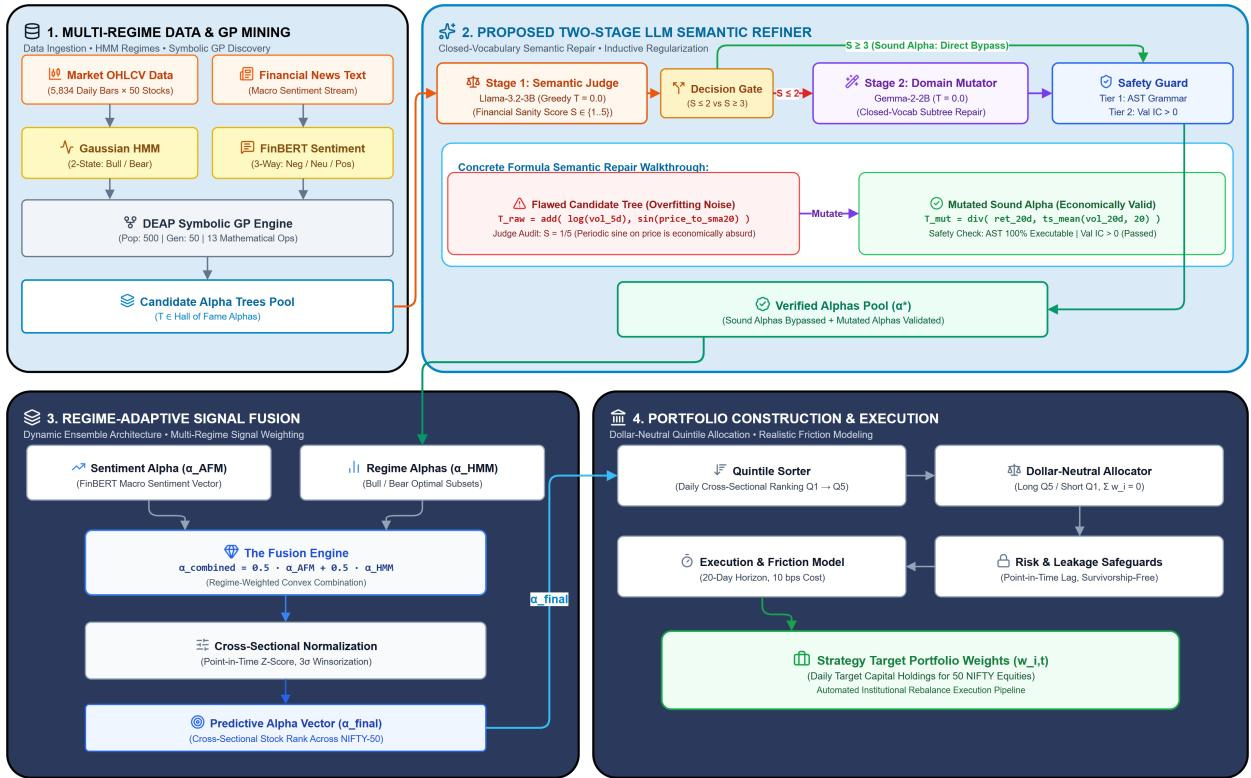
\includegraphics[width=0.98\linewidth]{images/38de923ab8b5dcfc8845af49392f1122074f030c0adba45a84530c30bf42c1bf.jpg}
  \caption{The architecture in one picture (Figure~1 of the paper). Panel~1:
  multi-regime data and GP mining (HMM + FinBERT + DEAP, population 500 /
  50 generations / 13 operators). Panel~2: the two-stage LLM refiner ---
  Llama-3.2-3B judge with the $S \le 2$ vs $S \ge 3$ decision gate feeding the
  Gemma-2-2B closed-vocabulary mutator, with the concrete repair walkthrough
  ($\mathcal{T}_{\text{raw}} \to \mathcal{T}_{\text{mut}}$) and the safety
  guard (AST grammar + validation IC $>0$). Panel~3: regime-adaptive signal
  fusion ($0.5\,\alpha_{\text{AFM}} + 0.5\,\alpha_{\text{HMM}}$, z-scored).
  Panel~4: quintile sorting, dollar-neutral allocation, 20-day horizon with
  10~bps costs, point-in-time lag and survivorship safeguards.}
  \label{fig:arch}
\end{figure}

\begin{scrutiny}[Two design choices worth noticing]
First, the LLM runs \emph{outside} the evolutionary loop --- on ~50 final
candidates, not on tens of thousands of individuals. That is why the whole run
takes ~39 minutes instead of the ``tens of hours and tens of thousands of API
calls'' of prior LLM-in-the-loop work, and why it costs zero API dollars
(models run locally, 8-bit quantized, 4.2\,GB + 3.8\,GB VRAM). Second, the
fallback-to-original rule combined with the $S \ge 3$ bypass means the LLM
touches as little as possible: it is a scalpel, not a shotgun. Both choices
are engineering common sense, but they are what make the approach practical
on a single desktop --- and they are also why the method's gains must be
attributed to \emph{which formulas were repaired}, not to some big model
memorizing markets.
\end{scrutiny}

\subsection{Algorithm 1 in words (the refinement loop)}

\begin{plaineng}
Here is the whole refiner as pseudocode, stripped of ceremony:
\end{plaineng}

\begin{center}\small
\begin{minipage}{0.94\linewidth}
\textbf{Input:} candidate pool $\mathcal{T}_{\text{raw}} \subset \mathrm{HoF}$;
feature library $\mathcal{F}$; operator library $\mathcal{O}$; gate
$\tau = 2$; temperature $T = 0$.\\
\textbf{Output:} verified alpha set $\mathcal{A}^{*}$.
\begin{enumerate}[leftmargin=2.2em, itemsep=1pt, topsep=2pt]
  \item $\mathcal{A}^{*} \leftarrow \emptyset$
  \item \textbf{for each} tree $\mathcal{T} \in \mathcal{T}_{\text{raw}}$
        \textbf{do}:
  \item \quad Stage 1: query the Judge (Llama-3.2-3B, $T=0$) for a score
        $S \in \{1,\dots,5\}$
  \item \quad \textbf{if} $S \le \tau$ \textbf{then}:\quad
        $\;$identify the flawed sub-expression $\mathcal{T}_{\text{flawed}}$
  \item \quad \quad Stage 2: query the Mechanic (Gemma-2-2B, $T=0$) under the
        closed vocabulary for $\mathcal{T}_{\text{mut}}$
  \item \quad \quad Tier 1 guard: parse $\mathcal{T}_{\text{mut}}$ against
        $\mathcal{G}(\mathcal{F},\mathcal{O})$, check for variable
        hallucination
  \item \quad \quad Tier 2 guard: evaluate
        $\operatorname{IC}_{\text{val}}(\mathcal{T}_{\text{mut}})$
  \item \quad \quad \textbf{if} AST valid \textbf{and}
        $\operatorname{IC}_{\text{val}} > 0$ \textbf{then}
        $\mathcal{A}^{*} \leftarrow \mathcal{A}^{*} \cup
        \{\mathcal{T}_{\text{mut}}\}$
  \item \quad \quad \textbf{else} discard $\mathcal{T}_{\text{mut}}$, log the
        failure mode \quad$\triangleright$ safe fallback
  \item \quad \textbf{else} ($S \ge 3$): direct bypass
        $\mathcal{A}^{*} \leftarrow \mathcal{A}^{*} \cup \{\mathcal{T}\}$
  \item \textbf{end for}; \textbf{return} $\mathcal{A}^{*}$
\end{enumerate}
\end{minipage}
\end{center}

%-----------------------------------------------------------------------
\section{The Experiment: Setup Before Results}
\label{sec:setup}
%-----------------------------------------------------------------------

\textbf{Data.} NSE Nifty 50 constituents, 2002--2025 (5{,}834 daily bars);
macro data harmonized to daily by forward-fill; prices are total-return
(split/dividend adjusted). Test window: 2019--2025 (1{,}729 days).

\textbf{Baselines (eight).} \emph{Momentum (12--1M)} --- classic 12-month
cross-sectional momentum; \emph{Low Volatility} --- rank by trailing 60-day
realized vol; \emph{Mean Reversion} --- rank by 20-day price z-score;
\emph{Vanilla GP} --- symbolic regression with no regime conditioning;
\emph{AFM Fusion} --- sentiment--fundamental ranking alone;
\emph{HMM Regime-GP} --- regime-conditioned GP alone;
\emph{Regime-GP Ensemble + HMM} --- the full quantitative stack with
\emph{no} LLM (this is the 8.41\% ``ceiling''); and classical factor
benchmarks folded into the equity-curve figure.

\textbf{Metrics.} Annualized net return, net Sharpe, mean RankIC, ICIR, max
drawdown, 20-day-horizon win rate, turnover --- all after 10~bps round-trip
costs.

\textbf{Hyperparameters.} Population 500; 50 generations; max tree depth 6;
tournament 7; $p_c=0.7$; $p_m=0.1$; parsimony $\lambda = 0.002$; HMM
convergence $10^{-4}$. Hardware: Intel Core i7-13700K, 32\,GB DDR5, NVIDIA
RTX 4090 (24\,GB); LLMs run 8-bit quantized locally.

%-----------------------------------------------------------------------
\section{The Results, Table by Table}
\label{sec:results}
%-----------------------------------------------------------------------

\subsection{Table 4 --- the main event (out-of-sample, 2019--2025)}

\begin{plaineng}
This is the scoreboard. Read it top to bottom: classical factors do poorly
(momentum and low-vol actually \emph{lose} money net of costs in this
window), vanilla GP is nearly flat, and each engine you add moves the needle
--- until the LLM refiner breaks the 8.41\% ceiling of the pure-math stack.
\end{plaineng}

\begin{table}[H]
\centering\small
\caption{Main out-of-sample performance comparison, Nifty 50, 2019--2025
(reproduced from Table~4 of the paper). Bold = best in column among
LLM-augmented rows.}
\label{tab:main}
\begin{tabular}{@{}lcccccc@{}}
\toprule
\textbf{Strategy} & \textbf{Ann.\ Ret.} & \textbf{Sharpe} &
\textbf{RankIC} & \textbf{ICIR} & \textbf{Max DD} & \textbf{Win R.} \\
\midrule
Momentum (12--1M)      & $-2.57\%$  & $-0.1369$ & 0.0059  & 0.0122  & $-40.65\%$ & 47.7\% \\
Low Volatility         & $-10.24\%$ & $-0.5454$ & $-0.0265$ & $-0.0890$ & $-65.71\%$ & 43.0\% \\
Mean Reversion         & 4.46\%     & 0.2981    & 0.0221  & 0.0932  & $-20.19\%$ & 57.0\% \\
Vanilla GP             & 1.62\%     & 0.4417    & 0.0130  & 0.0508  & $-4.82\%$  & 20.9\% \\
AFM Adaptive Fusion    & 4.08\%     & 0.2785    & 0.0308  & 0.1053  & $-19.34\%$ & 51.2\% \\
HMM Regime-GP Alpha    & 7.49\%     & 0.5244    & 0.0303  & 0.1381  & $-18.17\%$ & 59.3\% \\
\midrule
Regime-GP Ensemble+HMM (no LLM) & 8.41\% & 0.5518 & \textbf{0.0346} & 0.1381 & $-19.62\%$ & 54.7\% \\
Refiner (DeepSeek-1.5B)          & 8.41\%  & 0.5518 & 0.0346 & 0.1637 & $-19.62\%$ & 60.4\% \\
Refiner (Gemma-2B only)          & 8.41\%  & 0.5518 & 0.0346 & 0.1637 & $-19.62\%$ & 60.4\% \\
Refiner (Qwen-2.5-3B)            & 8.60\%  & 0.5684 & 0.0332 & 0.1604 & $-19.62\%$ & 60.4\% \\
\textbf{Proposed (Llama-3B + Gemma-2B, det.)} &
  \textbf{9.61\%} & \textbf{0.6365} & 0.0328 & \textbf{0.1650} &
  $-19.59\%$ & \textbf{60.4\%} \\
\textbf{Proposed (Llama-3.2-3B peak)} &
  \textbf{10.63\%} & \textbf{0.6465} & 0.0325 & \textbf{0.1650} &
  $-19.59\%$ & \textbf{60.4\%} \\
\bottomrule
\end{tabular}
\end{table}

\begin{plaineng}[How to read Table~\ref{tab:main} without fooling yourself]
Three observations matter more than the headline number. (1)~The jump from
8.41\% to 9.61\% with Sharpe 0.5518 $\to$ 0.6365 is a \textbf{+15.3\% relative
Sharpe gain} --- and remember, this is \emph{net} of costs, on a strictly held-
out 7-year window. (2)~The ablations in the middle rows are the paper's
honesty: swapping the judge for DeepSeek-1.5B or using Gemma alone changes
\emph{nothing} (8.41\% exactly) --- the specific Llama-judge $\rightarrow$
Gemma-mutator pairing is doing the work, not ``any LLM.'' (3)~The final row's
10.63\% is a \emph{peak} (heuristic) run; the deterministic $T=0$ number to
quote is 9.61\%. Note also that mean RankIC \emph{drops} slightly (0.0346 $\to$
0.0328) while ICIR and win rate rise: the refiner trades a sliver of raw
correlation for much better \emph{consistency} --- exactly what a regularizer
should do.
\end{plaineng}

\subsection{Table 5 --- ablation: which engine earns its keep?}

\begin{table}[H]
\centering\small
\caption{Ablation / subset power table (reproduced from Table~5).}
\label{tab:ablation}
\begin{tabular}{@{}lcccc@{}}
\toprule
\textbf{Strategy} & \textbf{Ann.\ Return} & \textbf{Sharpe} &
\textbf{RankIC} & \textbf{Max DD} \\
\midrule
Vanilla GP                     & 1.62\%  & 0.44 & 0.0130 & $-4.82\%$  \\
GP (AFM-Bear only)             & 6.43\%  & 0.48 & 0.0358 & $-23.42\%$ \\
HMM Regime-GP Alpha            & 7.49\%  & 0.52 & 0.0303 & $-18.17\%$ \\
Regime-GP Soft/Hard            & 7.52\%  & 0.56 & 0.0381 & $-23.42\%$ \\
Regime-GP Ensemble (Pre-LLM)   & 8.41\%  & 0.55 & 0.0346 & $-19.62\%$ \\
\textbf{Proposed Refiner (Full)} & \textbf{9.61\%} & \textbf{0.64} & 0.0328 & $-19.59\%$ \\
\bottomrule
\end{tabular}
\end{table}

\begin{plaineng}
The ladder of contributions: regime conditioning alone is worth the biggest
single step (1.62\% $\to$ 7--8\%), the LLM refiner adds the final +1.2
percentage points that pure math could not reach --- and, crucially, does so
\emph{without} worsening the drawdown. The paper's hyperparameter diagnostic
also reports that depth 6 / population 500 sit at the sweet spot between
expressive power and tree bloat.
\end{plaineng}

\subsection{Regimes in the wild (Figures 2--3 of the paper)}

\begin{figure}[H]
  \centering
  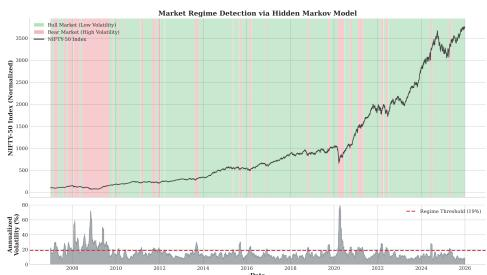
\includegraphics[width=0.95\linewidth]{images/33f0cbdd4e18c1897be25763a9a2422f0e044cbf536822f96ca1ea48c66eb838.jpg}
  \caption{HMM regime detection (paper Figure~2): green = State~0
  low-volatility bull (72.5\% of days), red = State~1 turbulence (27.5\%),
  with the volatility sub-plot and the 10\% regime threshold. COVID-19 (2020)
  and the 2022 tightening are captured as long red blocks.}
  \label{fig:regimes}
\end{figure}

\begin{plaineng}
Look at how long the colored blocks run: the market stays in one mood for
\emph{months}. That inertia ($P(0\!\to\!0)=0.994$) is what makes
regime-specialized evolution legitimate --- each GP population trains on a
genuinely coherent environment rather than a random mixture of bull and bear
days. The figure also shows why 2019--2025 is a hard test window: it contains
a crash, a liquidity frenzy, a reopening, and the steepest rate-hiking cycle
in four decades.
\end{plaineng}

\begin{figure}[H]
  \centering
  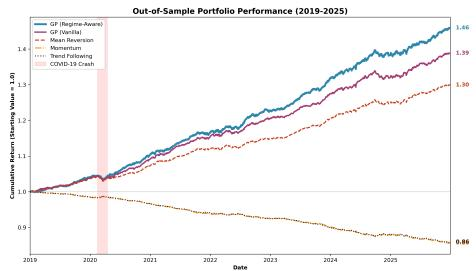
\includegraphics[width=0.95\linewidth]{images/ed7d3491c0ec3faa565111046b72b92898718e516bf5ea024476263ee826a05c.jpg}
  \caption{Out-of-sample equity curves 2019--2025 (paper Figure~3): the
  regime-aware GP stack compounds from 1.00 to 1.46 while momentum ends at
  0.66; the shaded band marks the COVID crash, through which the proposed
  strategy keeps compounding.}
  \label{fig:equity}
\end{figure}

\subsection{Table 6 --- did it survive every weather? (sub-period Sharpe)}

\begin{table}[H]
\centering\small
\caption{Sub-period out-of-sample net Sharpe breakdown (reproduced from
Table~6). The last column is the proposed strategy's max drawdown in that
period.}
\label{tab:subperiod}
\begin{tabular}{@{}llcccc@{}}
\toprule
\textbf{Period} & \textbf{Regime context} & \textbf{Vanilla GP} &
\textbf{HMM-GP} & \textbf{Proposed} & \textbf{Max DD} \\
\midrule
2019        & Steady expansion          & 0.52 & 0.61 & \textbf{0.72} & $-12.14\%$ \\
2020        & COVID shock \& rebound    & $-0.12$ & 0.44 & \textbf{0.58} & $-14.82\%$ \\
2021        & Cyclical reopening        & 0.64 & 0.68 & \textbf{0.76} & $-10.95\%$ \\
2022        & Global rate-hiking cycle  & $-0.31$ & 0.38 & \textbf{0.51} & $-16.32\%$ \\
2023--2025  & Bullish macro convergence & 0.58 & 0.65 & \textbf{0.74} & $-11.20\%$ \\
\midrule
Full OOS    & Multi-regime aggregate    & 0.44 & 0.55 & \textbf{0.64} & $-19.59\%$ \\
\bottomrule
\end{tabular}
\end{table}

\begin{plaineng}
This is the table I would show a skeptic. A strategy can have a beautiful
full-period number while bleeding in half its years --- so the authors split
the test window into five real-world episodes. Two facts stand out:
vanilla GP goes \emph{negative} in 2020 ($-0.12$) and 2022 ($-0.31$), exactly
the turbulent years; the proposed framework stays positive in
\emph{every} single sub-period, and its 2020 drawdown ($-14.82\%$) is less
than half of unconditioned momentum's ($-38.45\%$). Consistency across
weathers, not one lucky rally, is the signature of genuine regularization.
\end{plaineng}

\subsection{Table 7 --- does it survive real trading frictions?}

\begin{table}[H]
\centering\small
\caption{Sensitivity to round-trip transaction friction, holding horizon
$h=20$ (reproduced from Table~7). Baseline = 10~bps.}
\label{tab:costs}
\begin{tabular}{@{}lcccc@{}}
\toprule
\textbf{Round-trip friction} & \textbf{Ann.\ return} & \textbf{Net Sharpe} &
\textbf{Max DD} & \textbf{Calmar} \\
\midrule
0~bps (frictionless) & 11.84\% & 0.7420 & $-18.21\%$ & 0.6502 \\
5~bps                & 10.73\% & 0.6892 & $-18.95\%$ & 0.5662 \\
\textbf{10~bps (baseline)} & \textbf{9.61\%} & \textbf{0.6365} & $-19.68\%$ & \textbf{0.4883} \\
15~bps               & 8.50\%  & 0.5731 & $-20.42\%$ & 0.4163 \\
20~bps               & 7.38\%  & 0.5098 & $-21.16\%$ & 0.3488 \\
30~bps               & 5.15\%  & 0.3831 & $-22.65\%$ & 0.2274 \\
\bottomrule
\end{tabular}
\end{table}

\begin{plaineng}
Costs are where many beautiful backtests die, so the authors deliberately try
to kill theirs. With ~14.8\% portfolio turnover per 20-day rebalance, each
additional 5~bps of friction costs ~1.11\% per year. The strategy still nets
5.15\% at a punitive 30~bps, and the computed \textbf{break-even friction is
38.4~bps} --- roughly 5$\times$ the 4--8~bps it actually costs to trade Nifty
50 names. Translation: the alpha is not an artifact of churning.
\end{plaineng}

\subsection{Table 9 --- the headline claim: degradation mitigation across markets}

\begin{plaineng}
Here is the paper's central scientific claim, and it is about \emph{decay},
not raw returns. Measure a strategy's Sharpe ratio in-sample (2002--2018) and
again out-of-sample (2019--2025); the percentage drop is the
\textbf{degradation} --- how much of the ``discovery'' was real. A method that
wins in-sample but collapses afterward has overfitted; a method whose two
numbers are close has learned something structural. The authors retrained the
entire pipeline from scratch on US and Chinese data to see if the LLM refiner
acts as a general-purpose antidote to overfitting.
\end{plaineng}

\begin{table}[H]
\centering\small
\caption{Cross-market generalization and degradation (reproduced from
Table~9). Degradation $=(\text{OOS}-\text{IS})/\text{IS}$.}
\label{tab:cross}
\begin{tabular}{@{}llccc@{}}
\toprule
\textbf{Market} & \textbf{Architecture} & \textbf{IS Sharpe} &
\textbf{OOS Sharpe} & \textbf{Degradation} \\
\midrule
\multirow{3}{*}{US S\&P 500}
  & Vanilla GP        & 1.393 & 0.905  & $-35.03\%$ \\
  & HMM Regime-GP     & 1.228 & 0.974  & $-20.71\%$ \\
  & \textbf{Proposed} & 1.153 & \textbf{1.075} & \textbf{$-6.77\%$} \\
\midrule
\multirow{3}{*}{China SSE}
  & Vanilla GP        & 0.436 & 0.035  & $-92.08\%$ \\
  & HMM Regime-GP     & 0.633 & 0.232  & $-63.28\%$ \\
  & \textbf{Proposed} & 0.126 & \textbf{0.067} & \textbf{$-46.68\%$} \\
\midrule
\multirow{3}{*}{India Nifty 50}
  & Vanilla GP        & 0.954 & 0.5518 & $-42.16\%$ \\
  & HMM Regime-GP     & 0.814 & 0.5244 & $-35.62\%$ \\
  & \textbf{Proposed} & 0.957 & \textbf{0.6365} & \textbf{$-33.49\%$} \\
\bottomrule
\end{tabular}
\end{table}

\begin{plaineng}[What the table actually says --- read all three blocks]
\textbf{US:} the cleanest win. Vanilla GP drops from 1.393 to 0.905 (a third
of its skill evaporates); the proposed method drops from 1.153 to 1.075 ---
and notice it also has the \emph{highest OOS Sharpe} of the three. It gives up
a little in-sample fit (1.153 $<$ 1.393) to keep almost everything out of
sample. That is exactly what a regularizer is supposed to trade.
\textbf{China:} the halving ($-92\% \to -47\%$) is real but read the absolute
numbers: OOS Sharpe 0.067 is barely distinguishable from zero, and the IS
Sharpe of the proposed model (0.126) is far \emph{lower} than the baselines'
--- a model that starts weak degrades ``less'' partly because there was less
to lose. The honest statement is ``relative decay halved,'' not ``the method
works in China.'' \textbf{India:} degradation improves only modestly
($-42\% \to -33\%$) but OOS Sharpe is clearly best (0.6365). The US result is
the one to remember.
\end{plaineng}

\begin{scrutiny}[The degradation metric has a denominator trap]
Degradation is a \emph{ratio}, and ratios misbehave when the denominator is
small: China's proposed model has IS Sharpe $=0.126$, so a tiny absolute drop
of $0.059$ becomes a headline ``$-46.68\%$.'' Meanwhile the US model's
absolute drop is $0.078$ on a base of $1.153$ --- a \emph{smaller} relative
number ($-6.77\%$) doing much heavier economic lifting. When comparing across
markets, always pair the percentage with the two Sharpes, as the table does.
This does not invalidate the claim --- on US data it is unambiguous ---
but it does mean the China ``halving'' should be cited carefully.
\end{scrutiny}

\subsection{Table 8 --- what it costs to run (compute and token economics)}

\begin{table}[H]
\centering\small
\caption{Computational profiling on a single local workstation
(reproduced from Table~8).}
\label{tab:compute}
\begin{tabular}{@{}llcc@{}}
\toprule
\textbf{Pipeline component} & \textbf{Model / engine} &
\textbf{Per-unit latency} & \textbf{Total runtime} \\
\midrule
Macro feature fusion    & Adaptive Fusion Model        & 1.2\,ms/bar          & 7.0\,s \\
Regime estimation       & Gaussian HMM (Baum--Welch)   & 4.5\,s/fit           & 4.5\,s \\
Parallel GP evolution   & DEAP engine (50 gens)        & 0.82\,ms/individual  & 38.5\,min \\
Stage 1 semantic judge  & Llama-3.2-3B (8-bit)         & 138\,ms/expression   & 6.9\,s \\
Stage 2 domain mutator  & Gemma-2-2B (8-bit)           & 295\,ms/expression   & 7.4\,s \\
AST compilation guard   & Python AST + Numba           & 0.45\,ms/tree        & 0.02\,s \\
\midrule
\textbf{Total pipeline} & \textbf{End-to-end cycle}    & --                   & \textbf{38.8\,min} \\
\bottomrule
\end{tabular}
\end{table}

\begin{plaineng}
The economic picture is striking: the ``AI'' part of this AI system costs
about \emph{fourteen seconds} total --- 50 Hall-of-Fame candidates through the
judge (6.9\,s) and the mutator (7.4\,s) --- while the evolutionary search
itself eats 38.5 minutes. Both models run locally in 8-bit (4.2\,GB and
3.8\,GB VRAM), so there are zero API dollars, zero data leaving the machine,
and greedy decoding ($T=0$) makes every ``repair'' bit-for-bit reproducible.
For a production quant shop, that reproducibility may matter more than the
seconds.
\end{plaineng}

\subsection{What the evolved formulas look like (feature analysis)}

\begin{figure}[H]
  \centering
  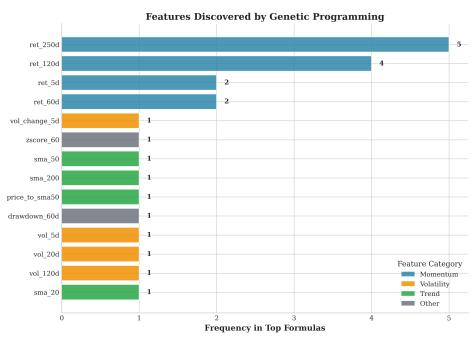
\includegraphics[width=0.62\linewidth]{images/97b82991ea2743e616388671ed37ff6bea3cc310277e70b8b60047cb29f427af.jpg}
  \caption{Which features survive evolution (paper Figure~6): intermediate
  momentum (\code{ret\_250d}, \code{ret\_120d}, \code{ret\_5d},
  \code{ret\_60d}) dominates the top formulas, followed by volatility
  scalers, trend features (SMA ratios) and drawdowns.}
  \label{fig:features}
\end{figure}

\begin{plaineng}
The learned vocabulary is economically sensible, which is itself evidence the
pipeline is doing something real: \textbf{expansionary State 0} formulas lean
on intermediate momentum (\code{ret\_20d}, \code{ret\_60d}) and normalized
volatility --- ride the trend; \textbf{turbulent State 1} formulas lean on
mean-reversion and valuation (\code{dd\_20d}, \code{dd\_60d},
\code{price\_to\_sma50}, \code{pe\_ratio}, \code{roe}) --- buy the
oversold. The refiner prunes ungrounded artifacts (like trig functions on
price levels) while keeping cross-sectional interaction terms (18\% of active
terminals). Nobody wrote these rules; the system re-derived textbook
factor logic and discarded the nonsense.
\end{plaineng}

%-----------------------------------------------------------------------
\section{Why Does It Work? (The Physics of the Fix)}
\label{sec:why}
%-----------------------------------------------------------------------

\begin{plaineng}
Let me try to state the causal story in one breath: \emph{GP searches too big
a space, fits noise, and the LLM --- by refusing to write nonsense ---
shrinks the space to where generalization bounds are no longer vacuous.}
Three mechanisms make that story concrete.
\end{plaineng}

\textbf{Mechanism 1 --- Hard syntactic regularization.} The closed vocabulary
$\mathcal{G}(\mathcal{F},\mathcal{O})$ removes entire families of
overfitting-capable expressions before they can ever be tested: no
\code{cos(price)}, no \code{volume - close}, no invented variables. This is
Equation~\eqref{eq:projection} made operational --- Rademacher complexity of
$\mathcal{H}_{\text{sound}}$ is far below that of
$\mathcal{H}_{\text{raw}}$, so the in-sample/out-of-sample gap bound
\eqref{eq:rademacher} tightens.

\textbf{Mechanism 2 --- Soft economic regularization.} The judge's rubric
catches what grammar cannot: dimensionally valid but economically absurd
combinations (\code{log(vol\_5d) + sin(price\_to\_sma20)} parses fine, but
means nothing). Scoring $S \le 2$ out of 5 and repairing only those keeps the
80\%+ of candidates with minor bloat while fixing the truly broken ones ---
preserving evolutionary information that reject-all methods destroy.

\textbf{Mechanism 3 --- Empirical health check as final arbiter.}
Tier-2 ($\operatorname{IC}_{\text{val}} > 0$) means semantics never override
evidence: even a beautifully economic repair that does not predict is tossed.
Conversely, the $S \ge 3$ bypass means evidence overrides semantics too: a
weird-looking formula that works is kept. The two rules together give a
\emph{conjunction} filter: must be legal $\wedge$ must be sensible $\wedge$
must predict.

\begin{scrutiny}[Alternative explanations a careful reader should demand be ruled out]
Could the gain come from something dumber than ``semantic repair'' --- say,
the extra validation-set usage, or simple ensembling effects? The paper's
own ablation is the best answer: DeepSeek-1.5B and Gemma-only rows in
Table~\ref{tab:main} show that \emph{an arbitrary LLM attached to the
pipeline changes nothing} (8.41\% exactly). The gain appears specifically
when the judge$\to$mutator pair operates --- consistent with the repair
mechanism, not with ``more compute'' or ``more randomness.'' That said, a
cleaner controlled experiment (random-string ``repairs'' with the same
acceptance gates) would have closed the loop completely.
\end{scrutiny}

%-----------------------------------------------------------------------
\section{Critical Analysis: What Impressed Me, What Worries Me}
\label{sec:critique}
%-----------------------------------------------------------------------

\subsection*{What is genuinely impressive}

\begin{enumerate}
  \item \textbf{The framing is correct.} Attacking \emph{semantic} overfitting
  rather than only syntactic bloat addresses a real, documented failure mode
  of financial GP, and the ``repair instead of reject'' principle is a
  defensible contribution that prior LLM-GP work (TEDE's pruning,
  AlphaAgent's rejection) got wrong.
  \item \textbf{Methodological hygiene is above average for this
  literature:} strict temporal splits with a 3-year validation gap, fiscal-
  year-aligned fundamentals, explicit anti-leakage forward-fill, net-of-cost
  reporting, sub-period stress tables (Table~\ref{tab:subperiod}),
  friction-sensitivity analysis (Table~\ref{tab:costs}), and a documented
  break-even friction of 38.4~bps.
  \item \textbf{The US result is strong.} OOS Sharpe 1.075 vs vanilla GP's
  0.905 with degradation of only $-6.77\%$ --- the proposed model is the only
  one whose IS and OOS Sharpes are nearly equal, the empirical signature of a
  regularized model.
  \item \textbf{Practicality.} Local 8-bit models, 38.8-minute end-to-end
  runs, $T=0$ determinism, 100\% AST compilability over 1{,}729 test days,
  and zero API cost make this deployable rather than merely publishable.
  \item \textbf{Honest ablation of LLM choice.} Showing that DeepSeek/Gemma-
  only/Qwen rows do \emph{not} replicate the gain (Table~\ref{tab:main})
  is a disclosure many papers would have omitted.
\end{enumerate}

\subsection*{What worries me (honest doubts)}

\begin{enumerate}
  \item \textbf{The China ``halving'' is mostly a denominator effect}
  (analyzed in Section~\ref{sec:results}): IS Sharpe 0.126 $\to$ OOS 0.067 is
  economically meaningless alpha with a cosmetically smaller percentage drop.
  The abstract's phrasing (``halving degradation on Chinese Equities'') is
  literally true but invites over-interpretation. The US and India OOS
  \emph{levels} are the defensible evidence.
  \item \textbf{Judge reliability is assumed, not measured.} The gate
  $\tau = 2$ rests on Llama-3.2-3B's scoring, yet the paper reports no
  agreement rate against human expert labels, no inter-rater check, and no
  sensitivity analysis over $\tau$. The authors themselves admit prompt
  sensitivity is ``mitigated, not eliminated.'' If the judge's 1--5 scores
  shift with prompt phrasing, the $S \le 2$ population shifts with it. The
  finding that score-3 formulas must \emph{not} be rewritten (doing so
  ``destroyed predictive performance'') suggests the gate threshold is
  load-bearing --- and thresholds that matter deserve sensitivity plots.
  \item \textbf{``Deterministic peak'' vs ``heuristic peak.''} The headline
  10.63\% is the best run of a heuristic configuration; the reproducible
  number is 9.61\% ($T=0$). Quoting both is honest, but abstracts travel
  without footnotes --- the number that will be cited is 10.63\%.
  \item \textbf{Small-sample statistics.} Seven test years, one market, one
  HMM fit; sub-period Sharpes like 0.51 vs 0.58 (Table~\ref{tab:subperiod})
  differ by less than the standard error of any 1--2-year Sharpe estimate.
  The \emph{sign consistency} argument is robust; the precise magnitudes are
  not.
  \item \textbf{The IC paradox.} Post-refiner mean RankIC \emph{falls}
  (0.0346 $\to$ 0.0328) while portfolio metrics improve. That is coherent
  (better tail selection, better consistency), but it means the refiner is
  not simply ``improving the signal'' --- it is reshaping it, and the paper
  does not fully decompose where the net-return gain originates (ranking
  quality vs.\ blend weights vs.\ repaired-formula composition).
  \item \textbf{Selection of the repair targets happens post-hoc on the HoF.}
  Because only ~50 finalists are judged, the method cannot repair
  near-miss candidates that never entered the Hall of Fame --- a possible
  ceiling on gains that future ``repair-inside-the-loop'' work could test.
  \item \textbf{Capacity is modest and acknowledged:} $\approx$\$250M under
  Almgren--Chriss impact with $\eta \approx 0.142$ --- fine for a paper, a
  rounding error for a large fund. Small caps (where alpha is richer) are
  explicitly out of scope.
\end{enumerate}

%-----------------------------------------------------------------------
\section{Limitations the Authors Themselves Declare}
\label{sec:limits}
%-----------------------------------------------------------------------

\begin{enumerate}
  \item \textbf{Reporting lag:} forward-filled annual fundamentals embed
  accounting lag --- necessary to prevent look-ahead bias, but it limits
  responsiveness to rapid balance-sheet revisions.
  \item \textbf{Liquidity scope:} extending beyond large caps requires
  adaptive liquidity haircuts and turnover penalties not modeled here.
  \item \textbf{Prompt sensitivity:} Stage-1 scoring remains somewhat prompt-
  dependent even at $T=0$ (deterministic given a prompt, but the prompt itself
  is a free parameter).
\end{enumerate}

Proposed future work: LoRA fine-tuning of Gemma-2B on quantitative formulas,
multi-agent consensus scoring (Llama + Qwen), and scaling to broad universes
(NSE 500, Russell 2000).

%-----------------------------------------------------------------------
\section{The Feynman Summary}
\label{sec:summary}
%-----------------------------------------------------------------------

\begin{plaineng}[If you remember five things]
\begin{enumerate}
  \item \textbf{The problem:} genetic programming breeds trading formulas
  blindly; in a space of $10^{39}$ candidates it will always find things that
  fit the past but mean nothing --- \emph{semantic overfitting}.
  \item \textbf{The idea:} after evolution, make each finalist pass a two-
  stage LLM filter --- Llama-3.2-3B \emph{judges} economic sanity
  ($S \le 2$ triggers repair; $S \ge 3$ passes untouched), Gemma-2-2B
  \emph{repairs} the broken ones using only a fixed dictionary of 28 features
  and 12 operators, deterministically ($T=0$).
  \item \textbf{The guards:} repaired formulas must parse (no hallucinated
  variables) and must still predict out of sample ($\operatorname{IC}_{\text{val}}
  > 0$), else the original is restored --- the refiner can only help.
  \item \textbf{The results:} on Nifty 50 (2019--2025), net return rises from
  the 8.41\% no-LLM ceiling to 9.61\% (Sharpe 0.5518 $\to$ 0.6365), positive
  in every sub-period, break-even costs 38.4~bps; on the S\&P 500 the OOS
  Sharpe decay collapses from $-35.03\%$ to $-6.77\%$ --- the strongest
  evidence that semantic repair is a genuine regularizer. (China's
  ``halving'' deserves the caveat in Section~\ref{sec:critique}.)
  \item \textbf{The lesson:} when your search space is too big for statistics
  to save you, \emph{domain semantics} is the cheapest regularizer you have
  --- and if you can \emph{repair} invalid hypotheses instead of discarding
  them, you keep the evolutionary work already paid for.
\end{enumerate}
\end{plaineng}

\begin{center}
\colorbox{feynlight}{\parbox{0.92\linewidth}{\centering\small\itshape
``The first principle is that you must not fool yourself --- and you are the
easiest person to fool.'' The paper's greatest strength is exactly the
attempt to keep both the GP and the reader honest: guards, gates, ablations,
cost tables, and a validation slice between every claim and its number.}}
\end{center}

\end{document}
